\documentclass[aspectratio=169,10pt]{beamer}

% ---------------------------------------------------------------
% Look: plain, flat, one accent colour
% ---------------------------------------------------------------
\usetheme{default}


\usepackage{booktabs}
\usepackage{tikz}
\usetikzlibrary{positioning,arrows.meta,calc}
\usepackage{pgfplots}
\pgfplotsset{compat=1.17}

\definecolor{accent}{HTML}{2A78D6}
\definecolor{muted}{HTML}{B9B8B3}
\definecolor{ink}{HTML}{1F1F1F}
\definecolor{quiet}{HTML}{5F5E5A}
\definecolor{tint}{HTML}{EEF4FC}

\setbeamertemplate{navigation symbols}{}
\setbeamercolor{frametitle}{fg=ink}
\setbeamerfont{frametitle}{size=\large,series=\bfseries}
\setbeamercolor{normal text}{fg=ink}
\setbeamercolor{itemize item}{fg=accent}
\setbeamertemplate{itemize items}[circle]
\setbeamertemplate{footline}{%
  \hfill\textcolor{quiet}{\tiny NHANES Aug 2021--Aug 2023 \quad \insertframenumber}\hspace{1em}\vspace{0.6em}}

\newcommand{\smallnote}[1]{{\scriptsize\color{quiet}#1}}

\begin{document}

% ===============================================================
% SLIDE 1 -- DATA CLEANING
% ===============================================================
\begin{frame}{Data cleaning: 11,933 NHANES participants $\rightarrow$ 2,794 in the analysis}

\begin{columns}[T,onlytextwidth]

% ---------- left: participant flow ----------
\begin{column}{0.47\textwidth}
\centering
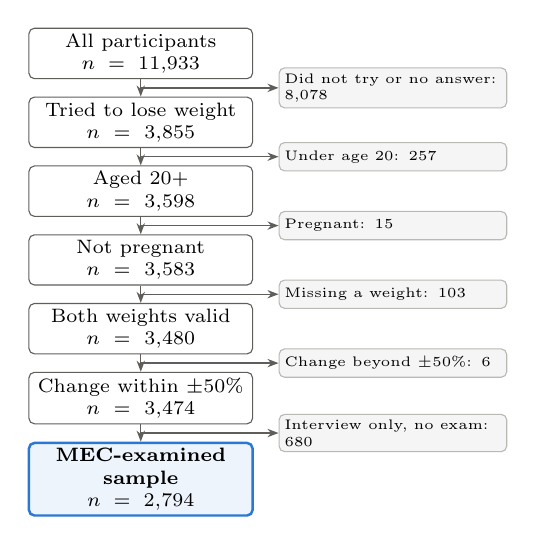
\begin{tikzpicture}[
  font=\scriptsize,
  stage/.style={draw=quiet, rounded corners=2pt, text width=2.7cm,
                minimum height=0.62cm, align=center, inner sep=2pt},
  final/.style={stage, draw=accent, fill=tint, line width=0.9pt, font=\scriptsize\bfseries},
  excl/.style={draw=muted, fill=gray!8, rounded corners=2pt, text width=2.75cm,
               minimum height=0.36cm, align=left, inner sep=2pt, font=\tiny},
  arr/.style={-{Stealth[length=4pt]}, draw=quiet, line width=0.5pt},
  node distance=0.22cm
]
\node[stage] (s0) {All participants\\ $n=11{,}933$};
\node[stage, below=of s0] (s1) {Tried to lose weight\\ $n=3{,}855$};
\node[stage, below=of s1] (s2) {Aged 20+\\ $n=3{,}598$};
\node[stage, below=of s2] (s3) {Not pregnant\\ $n=3{,}583$};
\node[stage, below=of s3] (s4) {Both weights valid\\ $n=3{,}480$};
\node[stage, below=of s4] (s5) {Change within $\pm$50\%\\ $n=3{,}474$};
\node[final, below=of s5] (s6) {MEC-examined sample\\ $n=2{,}794$};

\foreach \a/\b in {s0/s1, s1/s2, s2/s3, s3/s4, s4/s5, s5/s6}
  \draw[arr] (\a) -- (\b);

% exclusions, beside the gap between stages, all starting at the same x
\foreach \a/\b/\txt in {
  s0/s1/{Did not try or no answer: 8,078},
  s1/s2/{Under age 20: 257},
  s2/s3/{Pregnant: 15},
  s3/s4/{Missing a weight: 103},
  s4/s5/{Change beyond $\pm$50\%: 6},
  s5/s6/{Interview only, no exam: 680}}
{
  \coordinate (m) at ($(\a.south)!0.5!(\b.north)$);
  \node[excl, anchor=west] (e) at ($(m)+(1.75cm,0)$) {\txt};
  \draw[arr] (m) -- (e.west);
}
\end{tikzpicture}
\end{column}

% ---------- right: what was done ----------
\begin{column}{0.51\textwidth}
\footnotesize
\begin{itemize}\setlength{\itemsep}{2pt}
  \item \textbf{Merged 9 files} on \texttt{SEQN}: demographics, weight history,
        activity, diet, sleep, smoking, alcohol, PHQ-9, body measures (117 columns).
  \item \textbf{442 refused/don't-know codes $\rightarrow$ missing}, matched to answer
        length (7/9, 77/99, 777/999, 7777/9999); real 7s and 9s (e.g.\ 7~h sleep) kept.
  \item \textbf{Skip patterns filled, not imputed:} ``none'' $\rightarrow$ 0 or \emph{Never}
        (vigorous activity: 51.5\% $\rightarrow$ 0.5\% missing).
  \item \textbf{Derived:} activity min/week, sedentary h/day, PHQ-9 score,
        drinks/week, smoking status, sleep h/night, BMI 1 year ago.
  \item \textbf{Dropped:} child-only, admin and redundant columns, and
        post-change body size (outcome leakage).
\end{itemize}

\vspace{2pt}
\begin{beamercolorbox}[sep=4pt,rounded=true]{block body}
\footnotesize
\textbf{Outcome:} \% weight change $= (W_{\text{now}} - W_{\text{1 yr ago}}) / W_{\text{1 yr ago}} \times 100$\\[1pt]
\textbf{Features:} 15 covariates + 12 behaviors\\[1pt]
\smallnote{$\approx$12\% missing PHQ-9, drinks/week, income $\rightarrow$ multiple imputation; 2,117 complete cases (76\%).}
\end{beamercolorbox}
\end{column}

\end{columns}
\end{frame}

% ===============================================================
% SLIDE 2 -- EXPLORATION
% ===============================================================
\begin{frame}{Exploration: starting BMI dominates; behaviors are weak on their own}

\begin{columns}[T,onlytextwidth]

% ---------- left: outcome distribution ----------
\begin{column}{0.47\textwidth}
\centering
{\small\textbf{28\% lost $\geq$5\%; 22\% reported no change}}\\[1pt]
\smallnote{\% of adults by 1-year weight change (survey-weighted, $n=2{,}794$)}\\[2pt]
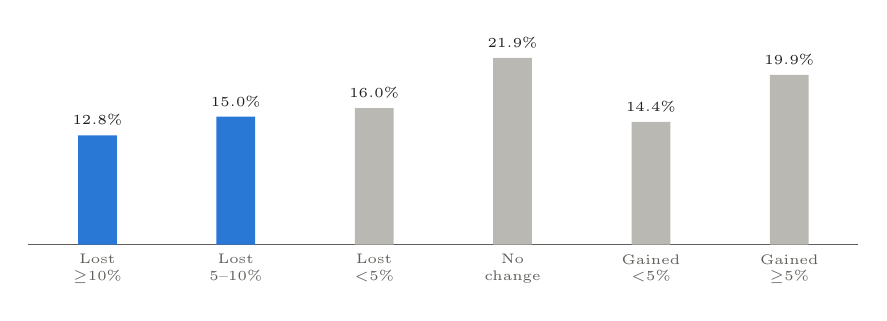
\begin{tikzpicture}
\begin{axis}[
  width=\linewidth, height=4.4cm,
  ybar, bar width=14pt, bar shift=0pt, ymin=0, ymax=26,
  axis x line*=bottom, axis y line=none,
  symbolic x coords={L10,L5,L0,N,G0,G5},
  xtick={L10,L5,L0,N,G0,G5},
  xticklabels={{Lost\\$\geq$10\%},{Lost\\5--10\%},{Lost\\$<$5\%},{No\\change},{Gained\\$<$5\%},{Gained\\$\geq$5\%}},
  xticklabel style={font=\tiny, align=center, text=quiet},
  nodes near coords={\pgfmathprintnumber[fixed,fixed zerofill,precision=1]{\pgfplotspointmeta}\%},
  nodes near coords style={font=\tiny, text=ink},
  enlarge x limits=0.10,
  axis line style={draw=quiet},
  major tick length=0pt,
]
\addplot[fill=accent, draw=none] coordinates {(L10,12.8) (L5,15.0)};
\addplot[fill=muted, draw=none] coordinates {(L0,16.0) (N,21.9) (G0,14.4) (G5,19.9)};
\end{axis}
\end{tikzpicture}

\vspace{2pt}
\smallnote{Weighted mean $-0.9\%$, median 0\%; 34\% gained. The spike at 0\% is heaping (same round number reported twice).}
\end{column}

% ---------- right: correlations ----------
\begin{column}{0.51\textwidth}
\centering
{\small\textbf{Correlation with \% weight change (Spearman $r$)}}\\[2pt]
\smallnote{negative = more weight loss \quad
  {\color{accent}$\blacksquare$} behavior \quad {\color{muted}$\blacksquare$} covariate}\\[2pt]
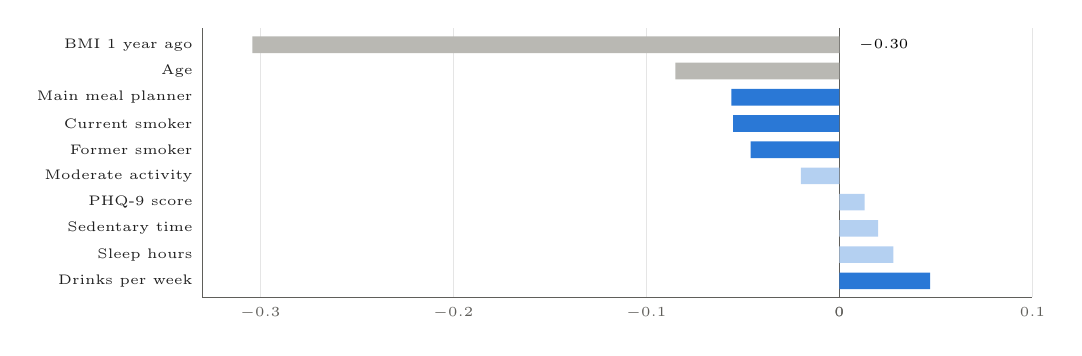
\begin{tikzpicture}
\begin{axis}[
  width=\linewidth, height=5.0cm,
  xbar, bar width=6pt, bar shift=0pt,
  xmin=-0.33, xmax=0.10,
  y dir=reverse,
  symbolic y coords={BMI 1 year ago,Age,Main meal planner,Current smoker,Former smoker,Moderate activity,PHQ-9 score,Sedentary time,Sleep hours,Drinks per week},
  ytick={BMI 1 year ago,Age,Main meal planner,Current smoker,Former smoker,Moderate activity,PHQ-9 score,Sedentary time,Sleep hours,Drinks per week},
  yticklabel style={font=\tiny, text=ink},
  xticklabel style={font=\tiny, text=quiet, /pgf/number format/fixed},
  xtick={-0.3,-0.2,-0.1,0,0.1},
  axis y line*=left, axis x line*=bottom,
  axis line style={draw=quiet},
  xmajorgrids, grid style={draw=gray!20},
  extra x ticks={0}, extra x tick style={grid style={draw=quiet}},
  major tick length=0pt,
  enlarge y limits=0.07,
]
\addplot[fill=muted, draw=none] coordinates {(-0.304,BMI 1 year ago) (-0.085,Age)};
\addplot[fill=accent, draw=none] coordinates {
  (-0.056,Main meal planner) (-0.055,Current smoker) (-0.046,Former smoker)
  (0.047,Drinks per week)};
\addplot[fill=accent!35, draw=none] coordinates {
  (-0.020,Moderate activity) (0.013,PHQ-9 score) (0.020,Sedentary time) (0.028,Sleep hours)};
\node[font=\tiny\bfseries, anchor=west] at (axis cs:0.005,BMI 1 year ago) {$-0.30$};
\end{axis}
\end{tikzpicture}

\smallnote{Faded = $p \geq 0.05$. No behavior exceeds $|r| = 0.06$; PHQ-9 and sleep look non-linear.}
\end{column}

\end{columns}

\vspace{4pt}
\begin{beamercolorbox}[sep=4pt,rounded=true]{block body}
\small\textbf{Next:} nested models (covariates vs.\ + behaviors) $\cdot$ LASSO + gradient boosting with SHAP
$\cdot$ lost $\geq$5\% as a second outcome $\cdot$ MEC exam weights
\end{beamercolorbox}

\end{frame}

\end{document}
